% !TEX TS-program = pdflatexmk
\documentclass[12pt]{article}

% Layout.
\usepackage[top=.75in, bottom=0.75in, left=.75in, right=.75in, headheight=1in, headsep=6pt]{geometry}

% Fonts.
\usepackage{mathptmx}
\usepackage[scaled=0.86]{helvet}
\renewcommand{\emph}[1]{\textsf{\textbf{#1}}}

% Misc packages.
\usepackage{amsmath,amssymb,latexsym}
\usepackage{graphicx,tikz}
\usepackage{array}
\usepackage{xcolor}
\usepackage{multicol}
\usepackage{tabularx,colortbl}
\usepackage{enumitem}
%to make tikz pics work
\usepackage{tikz,pgfplots}
\usetikzlibrary{arrows}
\newcommand{\midarrow}{\tikz \draw[-triangle 90] (0,0) -- +(.1,0);}

\usepackage[colorlinks=true]{hyperref}

% Paragraph spacing
\parindent 0pt
\parskip 6pt plus 1pt
\def\tableindent{\hskip 0.5 in}
\def\ts{\hskip 1.5 em}

\usepackage{fancyhdr}
\pagestyle{fancy} 
\lhead{\large\sf\textbf{MATH 663 }}
\rhead{\large\sf\textbf{Fall 2023}}
\chead{\large\sf\textbf{HW 9 }}

\newcommand{\localhead}[1]{\par\smallskip\textbf{#1}\nobreak\\}%
\def\heading#1{\localhead{\large\emph{#1}}}
\def\subheading#1{\localhead{\emph{#1}}}

%% Special Math Symbol shortcuts
\newcommand{\bbN}{\mathbb{N}}
\newcommand{\rad}{\text{rad}}
\newcommand{\diam}{\text{diam}}

%\newenvironment{clist}%
%{\bgroup\parskip 0pt\begin{list}{$\bullet$}{\partopsep 4pt\topsep 0pt\itemsep -2pt}}%
%{\end{list}\egroup}%

\usetikzlibrary{calc,arrows.meta}
%\pgfplotsset{my style/.append style={axis x line=middle, axis y line=
%middle, xlabel={$x$}, ylabel={$y$}, axis equal }}
\usetikzlibrary{arrows}
\newcommand{\marrow}{\tikz \draw[-triangle 90] (0,0) -- +(.1,0);}


\begin{document}
\begin{enumerate}
	\item In the network below, the capacity and flow value for each edge are represented with an ordered pair. Since the flow is everywhere zero, there is no need to direct the edges. However two edges are directed so you can see how to change the diagram.  Find a maximum flow from $s$ to $t$. Prove your answer is optimal by finding a cut with minimum capacity. \\
	
	
	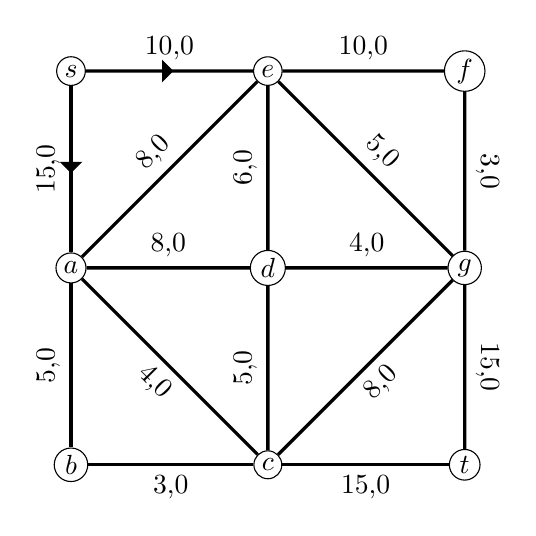
\begin{tikzpicture}[scale=2.5,every node/.style={draw,circle, inner sep=.05 cm}]
	
	\node (s) at (0,2){$s$};
	\node (a) at (0,1){$a$};
	\node (b) at (0,0){$b$};
	\node (c) at (1,0){$c$};
	\node (d) at (1,1){$d$};
	\node (e) at (1,2){$e$};
	\node (f) at (2,2){$f$};
	\node (g) at (2,1){$g$};
	\node (t) at (2,0){$t$};
	\begin{scope}[very thick, every node/.style={sloped,allow upside down}]
	%vertical edges
	\draw (s) -- node{\marrow} node[above,rotate=180]{15,0} (a);
	\draw (a) -- node[above,rotate=180]{5,0} (b);
	\draw (d) -- node[above,rotate=180]{5,0} (c);
	\draw (d) -- node[above]{6,0} (e);
	\draw (f) -- node[above,rotate=0]{3,0} (g);
	\draw (g) -- node[above,rotate=0]{15,0} (t);
	%horizontal edges
	\draw (s) -- node{\marrow} node[above]{10,0} (e);
	\draw (a) -- node[above]{8,0} (d);
	\draw (b) -- node[below]{3,0}  (c);
	\draw (e) -- node[above]{10,0} (f);
	\draw (d) -- node[above]{4,0} (g);
	\draw (c) -- node[below]{15,0}  (t);
	%diagonal edges
	\draw (a) -- node[above]{8,0} (e);
	\draw (a) -- node[below]{4,0}(c);
	\draw (e) -- node[above]{5,0} (g);
	\draw (c) -- node[below]{8,0} (g);
	\end{scope}
	\end{tikzpicture}

	
	\item Given $n \in \mathbb{N}$, find a capacity function for the network below such that the algorithm from the proof of the max-flow min-cut theorem (aka Ford-Fulkerson Theorem) will need more than $n$ augmenting paths if the algorithm consistently chooses the path badly.	\\
An \emph{augmenting} path is an $st$-path such that every (directed) edge on the path has available capacity. That is $c(\overrightarrow{e}) > f(\overrightarrow{e}).$ 
	
	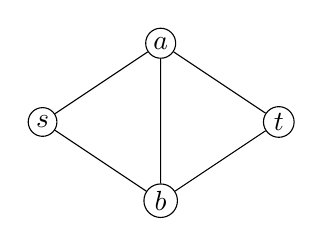
\begin{tikzpicture}[scale=1,every node/.style={draw,circle, inner sep=.05 cm}]
	\node (s) at (0,0){$s$};
	\node (a) at (1.5,1){$a$};
	\node (b) at (1.5,-1){$b$};
	\node (t) at (3,0){$t$};
	\draw (a)--(b)--(s)--(a)--(t)--(b);
	\end{tikzpicture}	
	
\item Use the max-flow min-cut theorem to prove part 1 of Corollary 3.3.5. (Copied below.)\\

\begin{quote}
Let $a$ and $b$ be two distinct vertices of the simple graph $G$. If $ab \not \in E,$ then the minimum number of vertices separating $a$ from $b$ is equal to the maximum number of independent $ab$-paths in $G.$
\end{quote}

\item Determine the value of $ex(n,K_{1,r})$ for all $r$ and $n$. (Assume that $n>r.$)
\item Show that every connected graph on at least three vertices contains a path or a cycle of length at least $\min\{2\delta, |G|\}.$
\item Prove the Erd\"{o}s-S\"os Conjecture for the case when the tree is a path. (Hint: use the previous problem.
\end{enumerate}
\end{document}